\documentclass[./../SoftwareEngineering.tex]{subfiles}

\section{Design Concepts}
Tập hợp các khái niệm (concept) thiết kế phần mềm cơ bản đều được triển khai khắp chiều dài lịch sử thiết kế phần mềm. Mặc dù mức độ phổ dụng của các phần mềm thao đổi qua từng năm, mỗi trong chúng đều đứng trước thử thách của thời gian. Mỗi người cung cấp thiết kế với nền móng đến từ nhiều phương pháp thiết kế tinh xảo (sophisticated) được áp dụng. Chúng có thể giúp bạn trả lời theo những câu hỏi dưới đây:

\begin{itemize}
	\item Các tiêu chuẩn để chia phần mềm thành các thành phần riêng lẻ?
	\item Làm thế nào để các hàm hoặc cấu trúc dữ liệu được phân chia chi tiết từ sự biểu diễn khái niệm của phần mềm?
	\item Các tiêu chuẩn xác định chất lượng kỹ thuật của một thiết kế phần mềm?
	
\end{itemize}

M. A. Jackson \cites{Jac75} từng nói: “The beginning of wisdom for a software engineer is to recognize the difference between getting a program to work, and getting it right.” tạm dịch "Sự khôn ngoan của kỹ sư phần mềm là xác định được sự khác biệt của một chương trình hoạt động và chương trình hoạt động hiệu quả." Các khái niệm thiết kế phần mềm cơ bản cung cấp một khung cần thiết giúp nó hoạt động "hiệu quả".


Ở phần dưới đây, tôi(tác giả) đưa ra cái nhìn cơ bản về các khái niệm thiết kế phần mềm quan trọng giữa các thiết kế phần mềm thiết kế truyền thống và phần mềm hướng đối tượng.

\subsection{Trừu tượng hóa (Abstraction)}
Khi bạn cân nhắc một giải pháp modular bất kỳ vấn đề nào, rất nhiều mức trừu tượng được đặt ra. Ở mức cao nhất của trừu tượng, một giải pháp được đưa ra rộng rãi là sử dụng ngôn ngữ của môi trường vấn đề(the language of the problem environment) (ngôn ngữ nghiệp vụ, ngôn ngữ người dùng). Ở các mức thấp hơn, một miêu tả chi tiết hơn của vấn đề được cung cấp. Thuật ngữ hướng vấn đề(problem-oriented) được ghép cặp với thuật ngữ  hướng hiện thực(implementation-oriented) trong sự nỗ lực đưa một giải pháp. Cuối cùng, ở mức thấp nhất, giải pháp được phát biểu thành một phương thức(manner) có thể hiện thực một cách trực tiếp. \cites{Vy08}


Ở mỗi mức trừu tượng được triển khai, bạn phải tạo ra sự trừu tượng cả thủ tục và dữ liệu. Trừu tượng thủ tục (procedural abstraction) ám chỉ đến một chuỗi chỉ thị có thể chỉ rõ chức năng và giới hạn. Thủ tục trừu tượng có thể bao hàm các các hàm đó, nhưng chi tiết được ẩn đi. Một ví dụ của trừu tượng hóa có thể là việc mở cửa. Việc mở được ấn đi bởi rất nhiều thủ tục(e.g. Đi tới cửa, vươn tới và giữ tay cầm, vặn tay cầm và đẩy cửa, đi qua cửa,vv...)


Trừu lượng dữ liệu(data abstraction) là tên của tập hợp dữ liệu được mô tả trong đối tượng. Ở ngữ cảnh của thủ tục mở cửa, bạn có thể định một dữ liệu trừu tượng gọi cửa (door). Như bất kỳ đối tượng dữ liệu khác, dữ liệu trừu tượng của door bao gồm một tập các thuộc thành mô tả được dữ liệu(e.g. kiểu của cửa, hướng gió, cách mỏ, khối lượng, kích thước). Nó theo bởi các thủ tục mở cần sử dụng thông tin của thuộc tính của kiểu Door.


\subsection{Kiến trúc (Architecture)}
Kiến trúc phần mềm ám chỉ tới "toàn thể cấu trúc của phần mềm và cách mà cấu trúc cung cấp sự thích hợp về mặt khái niệm của hệ thống".\cites{Sha95} Một cách đơn giản, kiến trúc là cấu trúc hoặc tổ chức của các thành phần cấu thành, cách thức các thành phần tương tác với nhau, và cấu trúc của dữ liệu sử dụng trong các thành phần cấu thành. Ở mức rộng, biểu diễn các phần lớn của hệ thống và cách thức tương tác của chúng.


Một mục tiêu của thiết kế phần mềm xuất hướng tới(to derive) một bản thiết kế kiến trúc(an architectural rendering) của hệ thống. Bản thiết kiến này như một kết cấu(framework) mà từ đó các thiết kế chi tiết được tiến hành. Tập hợp các mẫu kiến trúc được các kỹ sư phần mềm để giải quyết các vấn đề về thiết kế chung. 
Shaw and Gralan \cites{Sha95} giải thích cả đặc tính nên được định nghĩa như một phần của thiết kế hệ thống: 

\begin{description}
	\item [Structural properties.] Đây là một dạng biểu diễn của thiết kế kiến trúc định nghĩa các thành phần của hệ thống(e.g. modules, đối tượng, filter) và cách thức mà các thành phần đó được đóng gói và tương tác với nhau. Ví dụng: đối tượng được đóng gói cả dữ liệu và sự xử lý thông qua điều khiển và tưởng tượng dữ liệu bằng cách triển khai các phương thức.
	\item [Extra-functional properties.]  Mô tả thiết kế kiến trúc nên giải thích(should address) làm thế nào để kiến trúc có thể giải quyết các vấn đề về hiệu năng, công suất, độ tin cậy, bảo mật, khả năng thích nghi và các khía cạnh khác của hệ thống phần mềm.
	\item [Families of relate system.] Mô hình thiết kế nên phác thảo (should draw) các mẫu thiết kế lặp lại thường gặp trong thiết kế các họ hệ thống tượng tự (families of similar system). Trong đó, các thiết kế nên có khả năng tải sử dụng các khối kiến trúc.
\end{description}

các mô hình khác nhau \cites{Gar95}. Mô hình hướng cấu trúc (Structural models) biểu diễn kiến trúc như một tập tổ chức của các thành phần (component).Mô hình khung kiến trúc (Framework models) tăng các mức trừu tượng bằng cách cố gắng xác định các khung kiến trúc (architectural design framework) lặp lại giữa các ứng dụng tương tự nhau. Mô hình kiến trúc động (Dynamic models) giải quyết các khía cạnh về hành vi của kiến trúc, chúng cho biết cấu trúc hoặc cấu hình của hệ thống có thể thay đổi như một hàm hoặc các sự kiện bên ngoài. Mô hình quy trình (Process models) tập trung các thiết kế của doanh nghiệp hoặc các quy trình kỹ thuật mà hệ thống cần đáp ứng được. Cuối cùng là Mô hình chức năng  (Functional models) có thể sử dụng để biểu diễn sự phần cấp của hệ thống. 


Một số lượng Ngôn ngữ đặc tả kiến trúc (Architectural description language) (ADL) được phát triển để biểu diễn các mô hình đó \cites{Sha95b}. Mặc dù rất nhiều ngôn ngữ ADL được đưa ra, nhưng điểm chung được cung cấp được các thành phần hệ thống và cách thức chúng được kết nối với nhau.


Nên chú ý rằng có một số tranh cãi xung quanh vị trí của kiến trúc trong thiết kế. Một số nghiên cứu chỉ ra rằng sự phát sinh kiến trúc phần mềm nên tách biệt khỏi thiết kế và chúng nên xảy ra giữa yêu cầu kỹ thuật và các hành động thiết kế thông thường. Một số khác tin rằng các kiến trúc là một phần không thể thiếu của quá trình thiết kế. Điều này sẽ được bàn thêm ở chương 9.

\subsection{Pattern}
Bard Appleton định nghĩa mẫu thiết kế (a design pattern) theo định nghĩa: "A pattern is a named nugget of insight which conveys the essence of a proven solution to a recurring problem within a certain context amidst competing concerns” \cites{App00}. tạm dịch "Mẫu thiết kế là một giải pháp được đặt tên, chúng đã được chứng minh giải quyết được các vấn đề lặp lại trong các tình huống cụ thể". Hay nói một cách khác, mẫu thiết kế đưa ra nhưng một thiết kế cấu trúc giải quyết các vấn đề cụ thể trong tính huống cụ thể và trong đó ... có thể tác dụng đến cách áp dụng và sử dụng nó. (amid “forces” that may have an impact on the manner in which the pattern is applied and used.)


Ý nghĩa của mỗi mẫu thiết kế cung cấp chi tiết các người thiết kế xác định (1) mẫu thiết kế có thể áp dụng được hay không trong một trường làm việc hiện tại, (2) liệu có thể tái sử dụng chứng (từ đó tiết kiệm thời gian), và (3) liệu mẫu thiết kế có thể phục vụ một hướng dẫn trong các việc phát triển tương tự nhưng khác nhau về chức năng hoặc cấu trúc. Chi tiết sẽ được bàn luận thêm ở chương 12.


\subsection{Phân tách quan hệ} 
Sự phân tách quan hệ(separation of concern) là một khái niệm thiết kế \cites{Dij82} gợi ý một vấn đề phức nào cũng có thể xử lý một cách dễ dàng hơn nếu nó có thể chia thành các chi tiết(pieces) mà chúng có thể giải quyết hoặc/và tối ưu một cách độc lập. Một quan hệ là một tính năng hoặc hành vi được chỉ định như một phần của mô hình thiết kế. Bằng cách chia thành các chi tiết nhỏ hơn, các chi tiết dễ xử lý dễ hơn, các vấn đề ít rủi ro và mất ít thời gian để xử lý hơn.


Với hai vấn đề p1 và p2, nếu độ phức tạp của p1 lớn hơn độ phức tạp thì công sức bỏ ra để giải quyết p1 sẽ lớn hơn thời công sức bỏ ra để giải quyết p2. Ở các ca thông thường, một cách khách quan, sẽ mất nhiều thời gian hơn để giải quyết các vấn đề khó hơn.


Nó cũng đưa ra độ phức tạp của hai vấn đề khi ta kế hợp chủng thường lớn hơn tổng độ phức tạp khi mỗi vấn đề được chia tách. Nó dẫn đến tư tưởng chia-để-trị - một cách đơn giản để giải quyết các vấn đề nếu bạn chia thành các chi tiết dễ xử lý. Đây là điểm mấu chốt để có được một phần mềm có tính module cao hơn. 
Độ phức tạp có thể chỉ ra với phương trình: 
\begin{displaymath}
C(p_1+p_2) > C(p_1) + C(p_2) \text{ and } E(p_1+p_2) >E(p_1) + E(p_2)
\end{displaymath}
Trong đó C là hàm cảm nhận độ phức tạp của vấn đề và E là hàm nỗ lực để hoàn thành của vấn đề. 
Các khái niệm liên quan đến sự phân tách quan hệ được giải thích thêm ở các phần bên dưới đây.

\subsection{Module}
Module là một cách phổ biến để phân tách quan hệ. Phần mềm sẽ được chia thành các đơn vị có tên và địa chỉ thành phần xác định. Chúng được gộp lại để giải quyết vấn đề được đưa ra. 

Nó cũng được phát biểu rằng “modularity is the single attribute of software that allows a program to be intellectually manageable” \cites{Mye78} tạm dịch là "tỉnh module là thuộc tính riêng của phần mềm cho phép tổ chức một chương trình trở nên quản lý được theo một cách thông minh" \cites{Vy08}. Kỹ sư phần mềm không thể thể nắm bắt được một phần mềm nguyên khổi (i.e. một phần mềm được tổ chức như một module). Số lượng luồng điều khiển, biên độ tham chiếu (span of reference), số lượng các biến và độ phức tạp của phần mềm sẽ khiến việc hiểu được là điều dường như không thể. Trong phần lớn trường hợp, bạn nên chia thiết kế thành nhiều module khác nhau làm cho phần mềm dễ hiểu hơn và như một hệ quả, chi phí để hoàn thành phần mềm sẽ giảm.
\begin{figure}[!htb]
	\centering
	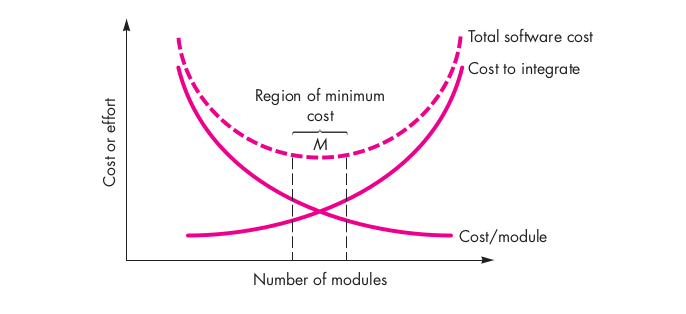
\includegraphics[width=\textwidth]{figure_8_2.png}
	\caption{Đồ thị tương quan giữa số moudle và chi phí}
	\label{ref: fig8_2}
\end{figure}

Như đã thảo luận ở các phần trước, nếu bạn chia các vấn đề đủ nhỏ thì chi phí sẽ không đáng kể, nhưng điều này thực tế là không thể!! Ở hình 8.2 [Reference to Figure 8.2] thì nỗ lực chia nhỏ phần mềm thành các module riêng rẻ sẽ làm số lượng module tăng theo. Với một tập yêu cầu, số lượng module nhiều lên tương đương việc kích thước module riêng lẻ sẽ nhỏ hơn, chi phí phát triển modul sẽ ít đi. Tuy nhiên, khi số lượng module tăng lên, nỗ lực kết hợp chúng thành hệ thống sẽ tăng. Nhưng đặc điểm này sẽ dẫn đến đường cong ở [Hình 8.2]. Như vậy, nếu có M modul thì kết quả sẽ đạt được chi phí tối thiểu, nhưng không đủ chính xác để để xác định giá trị M. Đường cong đưa ra ở [Hình 8.2] hữu ích khi xét đến tính modul của phần mềm. Bạn nên module hóa, nhưng nên ở trong cùng lân cận của M. Nên tránh các vùng undermodularity và overmodularity. Nhưng làm thế nào để xác định được vùng lân cận của M? Số lượng modul nên là bao nhiêu? Những câu hỏi này đòi hỏi khả năng hiểu của các khái niệm khác của chương này.


Bạn nên module hóa thiết kế(và chương trình đích) sẽ giúp lập trình viên dễ lên kế hoạch, chi phí phần mềm có thể xác định và phân phối, những thay đổi có thể dễ dàng xác định, kiểm thử và tìm lỗi sẽ hiệu quả hơn và lâu dài hơn là hệ thống được bảo trình liên tục mà không có các sự cố nghiêm trọng xảy ra.


\subsection{Che giấu thông tin (Data hiding)}
Khái niệm mô đun hóa dẫn ta tới một câu hỏi: "Làm cách nào để có thể chia một phần mềm thành bộ modun tốt nhất?". Nguyên tắc che giấu thông tin cho rằng các module nên được "characterized by design decisions that (each) hides from each other". Nói cách khác, mô đun nên được thiết kế sao cho thông tin (thuật toán và dữ liệu) nằm trong mô đun không thể được truy cập từ những mô đun khác không cần đến thông tin đó.


Che giấu cho rằng việc modun hóa hiệu quả có thể đạt được bằng cách định nghĩa một tập các modun độc lập, giao tiếp với nhau bằng lượng thông tin tối thiểu cần thiết để thực hiện chức năng của phần mềm. Quá trình trừu tượng hóa sẽ giúp định nghĩa các thực thể của phần mềm. Che giấu thông tin định nghĩa và áp đặt giới hạn truy cập (access constraint) tới những chi tiết cụ thể của module.


Việc áp dụng nguyên lý che dấu thông tin cho các hệ thống modular cung cấp lợi ích lớn nhất khi ta cần sửa đổi hệ thống trong quá trình kiểm thử và sau nữa là quá trình bảo trì. Vì dữ liệu và chi tiết thuật toán (procedural detail) của module được che giấu khỏi những phần khác của hệ thống, các lỗi xuất hiện khi sửa đổi sẽ khó lan ra những phần khác của hệ thống.

\subsection{Độc lập giữa các hàm}
Khái niệm độc lập chức năng được phát triển từ khái niệm separation of concerns, module hóa, trừu tượng hóa và che giấu thông tin. Trong bài luận bất hủ về thiết kế phần mềm, Wirth và Parnas chỉ ra những kĩ thuật để nâng cao tính độc lập của module. Một thời gian sau, công trình của Stevens, Myers và Constantine đã hoàn thiện khái niệm này.


Độc lập chức năng đạt được bằng việc phát triển các module với một chức năng duy nhất. Nói cách khác, bạn nên thiết kế phần mềm sao cho mỗi module xử lý một tập con các yêu cầu cụ thể và sở hữu một API đơn giản. Vậy tại sao độc lập tính năng lại quan trọng?


Phần mềm được module hóa hiệu quả (với các module độc lập) sẽ dễ dàng phát triển hơn. Vì chức năng có thể được chia nhỏ, đóng gói lại và API được đơn giản hóa. Module độc lập sẽ dễ dàng bảo trì (và kiểm thử) hơn vì tác dụng phụ do thiết kế hoặc do sửa đổi code bị giới hạn, ngăn lỗi của một phần ảnh hưởng tới các phần khác. Module độc lập còn giúp việc tái sử dụng dễ dàng hơn. Tóm lại, độc lập tính năng là chìa khóa dẫn tới thiết kế tốt, và thiết kế tốt là chìa khóa dẫn tới một phần mềm chất lượng.

\subsection{Refinement}
\subsection{Aspects}
\subsection{Refinement}
\subsection{Aspects}
\subsection{Refactoring}
An important design activity suggested for many agile methods (Chapter 3), refactoring is a reorganization technique that simplifies the design (or code) of a component without changing its function or behavior. Fowler [Fow00] defines refactoring in the following manner: “Refactoring is the process of changing a software system in such a way that it does not alter the external behavior of the code [design] yet improves its internal strúcture.”
\subsection{Object-Oriented Design Concepts}
\subsection{Design Classes}





